\clearpage
\appendix
\counterwithin{equation}{section}
\renewcommand{\theequation}{\thesection.\arabic{equation}}

\section{Proofs}
\label{app:proofs}

\subsection{Offspring and reporting model}
\label{app:model}

The negative binomial distribution $\NB(r,p)$ with $r$ successes and success probability $p$ has mean $r(1-p)/p$ and variance $r(1-p)/p^2$. Setting $r=k$ and $p=k/(k+R_t)$ gives Eq.~(\ref{eq:offspring}). A sum of $n$ independent $\NB(k,p)$ variables is $\NB(nk,p)$, and binomial thinning of $\NB(r,k/(k+\mu))$ with retention probability $\rho$ gives $\NB(r,k/(k+\rho\mu))$, which together give Eq.~(\ref{eq:observed}).

\subsection{The period-specific target}
\label{app:target1}

Write $c$ for an observed value of $C_t$. From Eq.~(\ref{eq:observed}), the log-likelihood of $R_t$ given $n$ is given by:
\begin{equation}
  \ell(R_t)=\text{const}+nk\log\frac{k}{k+\rho R_t}+c\log\frac{\rho R_t}{k+\rho R_t},
\end{equation}
and the score can be written as:
\begin{equation}
  \dot{\ell}(R_t)=\frac{c}{R_t}-\frac{(c+nk)\rho}{k+\rho R_t}=\mathcal{I}(R_t)\,(\Rhat_t-R_t),\qquad
  \mathcal{I}(R_t)=\frac{n}{R_t/\rho+R_t{}^2/k},
  \label{eq:score}
\end{equation}
where $\mathcal{I}(R_t)$ is the Fisher information. The conditional mean of $\Rhat_t=c/(\rho n)$ is $R_t$, and its conditional variance is $R_t/(\rho n)+R_t{}^2/(kn)=1/\mathcal{I}(R_t)$. Because the score in Eq.~(\ref{eq:score}) is proportional to $\Rhat_t-R_t$, the Cram\'er--Rao bound is attained for every finite $n$. The distribution in Eq.~(\ref{eq:observed}) is a one-parameter exponential family in $C_t$ with natural parameter $\log[\rho R_t/(k+\rho R_t)]$, which ranges over an open interval, so $C_t$ is complete and sufficient. By the Lehmann--Scheff\'e theorem, $\Rhat_t$ is the uniformly minimum-variance unbiased estimator of $R_t$ \citep{lehmann1998theory, lehmann2005testing}.

\subsection{Proof of Proposition~\ref{prop:average}}
\label{app:prop1}

Under H4, $\E(R_t\mid n)=\Rbar$ and $\Var(R_t\mid n)=v_R$. By the law of total variance and Appendix~\ref{app:target1}, the error variance is given by:
\begin{equation}
  \Var(\Rhat_t\mid n)=\E\!\left[\frac{R_t}{\rho n}+\frac{R_t{}^2}{kn}\right]+\Var(R_t)=v_R+\frac{\Rbar}{\rho n}+\frac{\Rbar^2+v_R}{kn},
\end{equation}
and substituting $m=\rho n$ gives Eq.~(\ref{eq:var-average}). Parts (i) and (ii) follow by taking limits. For part (iii), $[V(m)-V(2m)]/V(m)=[A/(2m)]/(v_R+A/m)=1/[2(1+m/\mx)]$, which equals one quarter at $m=\mx$. For part (iv), let $\tilde{\theta}$ be any estimator from data on period $t$ with $\E(\tilde{\theta}\mid R_t)=R_t$. Then $\E(\tilde{\theta}-\Rbar)^2=\E[\Var(\tilde{\theta}\mid R_t)]+v_R\ge\E[1/\mathcal{I}(R_t)]+v_R=V$, with equality for $\Rhat_t$. For one-step prediction of $y=C_{t+1}/m$ when $R_{t+1}$ is independent of the history, $\E(\hat{y}-y)^2=(\hat{y}-\E y)^2+\Var(y)\ge V$, with equality at $\hat{y}=\Rbar$.

The marginal effects of coverage and completeness are $-\partial V/\partial\log n=A/m$ and $-\partial V/\partial\log\rho=\Rbar/m$, so their ratio is $A/\Rbar$. If $R_t$ follows a stationary first-order autoregressive process with variance $v_R$ and autocorrelation $\phi$, the best linear predictor of $R_{t+1}$ given $R_t$ has error variance $(1-\phi^2)v_R$ \citep{hamilton1994time}. For $J$ jurisdictions with common variance $v_R$ and mean pairwise correlation $\bar{c}$, the variance of their average is $J^{-2}[Jv_R+J(J-1)\bar{c}v_R]$, which gives Eq.~(\ref{eq:pooling}).

\subsection{Proof of Proposition~\ref{prop:report-noise}}
\label{app:prop2}

Write $\sigma^2=\Var(p_t)=\tau^2\rho^2$. Given $(n,R_t,p_t)$, $C_t$ has mean $p_tnR_t$ and variance $p_tnR_t+p_t{}^2nR_t{}^2/k$. Averaging over $p_t$, the conditional variance given $(n,R_t)$ is given by:
\begin{equation}
  \Var(C_t\mid n,R_t)=\rho nR_t+\frac{(\rho^2+\sigma^2)nR_t{}^2}{k}+\sigma^2n^2R_t{}^2.
\end{equation}
The conditional mean is $\rho nR_t$, so $\Rhat_t$ remains unbiased for $\Rbar$. Averaging over $R_t$ and dividing by $(\rho n)^2$ gives:
\begin{equation}
  V_H(m)=v_R+\tau^2(\Rbar^2+v_R)+\frac{\Rbar}{m}+\frac{\rho(1+\tau^2)(\Rbar^2+v_R)}{km},
\end{equation}
which is Eq.~(\ref{eq:vH-AH}). Writing $U_0=\Rbar{}^2+v_R$ and $U=(1+\tau^2)U_0$, the limiting error variance is $v_R+v_H=U-\Rbar{}^2$ and $A_H=\Rbar+\rho U/k$, so the mean and variance of $\Rhat_t$ depend on $v_R$ and $\tau$ only through $U$. For the generalised balance scale, the algebraic difference satisfies
\begin{equation}
  m_{\times,H}-\mx = \frac{A_H}{v_R+v_H} - \frac{A}{v_R} = \frac{\tau^2 U_0\left(\frac{\rho v_R}{k}-A\right)}{v_R(v_R+\tau^2 U_0)}.
\end{equation}
Because $A=\Rbar+\rho U_0/k > \rho v_R/k$ for all $\Rbar>0$ and $k>0$, the bracketed term is strictly negative: $\rho v_R/k - A = -(\Rbar+\rho\Rbar^2/k)<0$. Thus $m_{\times,H}\le\mx$, with equality holding if and only if $\tau=0$, and strict inequality $m_{\times,H}<\mx$ holding whenever $\tau>0$.

\subsection{Proof of Proposition~\ref{prop:allocation}}
\label{app:prop3}

Conditional on $(R_1,\dots,R_T)$, counts in different periods are independent. With $\bar{R}_T=T^{-1}\sum_tR_t$, the variance of the mean estimate is given by:
\begin{equation}
  \Var\!\Big(\frac{1}{T}\sum_{t=1}^T\Rhat_t\Big)=\Var(\bar{R}_T)+\frac{A}{Tm},
\end{equation}
where $\Var(\bar{R}_T)=v_R/T$ for independent periods, giving Eq.~(\ref{eq:alloc-indep}). For a stationary first-order autoregressive process with $\Cov(R_s,R_t)=v_R\phi^{|s-t|}$, $T^2\Var(\bar{R}_T)=v_R[T+2\sum_{h=1}^{T-1}(T-h)\phi^h]$, and summing the geometric series gives Eq.~(\ref{eq:ar-sum}) \citep{hamilton1994time}. Substituting $T=\mathcal{B}/(c_0+c_1m)$ into Eq.~(\ref{eq:alloc-indep}) gives the objective:
\begin{equation}
  f(m)=\frac{(c_0+c_1m)(v_R+A/m)}{\mathcal{B}}=\frac{c_0v_R+c_1A+c_1v_Rm+c_0A/m}{\mathcal{B}},
\end{equation}
which is strictly convex for $c_0>0$, with $f'(m)=(c_1v_R-c_0A/m^2)/\mathcal{B}$. The unique stationary point is $m^{*2}=c_0A/(c_1v_R)=(c_0/c_1)\mx$, which is Eq.~(\ref{eq:optimal-m}).

\subsection{Proof of Corollary~\ref{cor:switch}}
\label{app:cor1}

Write $U_0=\Rbar^2+v_R$. From Eq.~(\ref{eq:vH-AH}), the gains from proportional increases in coverage and completeness are given by:
\begin{equation}
  -\frac{\partial V_H}{\partial\log n}=\frac{\Rbar}{\rho n}+\frac{(1+\tau^2)U_0}{kn},\qquad
  -\frac{\partial V_H}{\partial\log\rho}=\frac{\Rbar}{\rho n}-\rho\frac{\mathrm{d}\tau^2}{\mathrm{d}\rho}\,U_0\left(1+\frac{1}{kn}\right).
\end{equation}
If $\mathrm{d}\tau^2/\mathrm{d}\rho=0$, the first gain exceeds the second by $(1+\tau^2)U_0/(kn)>0$. Under binomial sampling of $\nu$ units, $\Var(p_t)=\rho(1-\rho)/\nu$, $\tau^2=(1-\rho)/(\rho\nu)$ and $\rho\,\mathrm{d}\tau^2/\mathrm{d}\rho=-1/(\rho\nu)$. The second gain minus the first is
\begin{equation}
  \frac{U_0}{kn}\left[\frac{kn+\rho}{\rho\nu}-1\right],
\end{equation}
which is positive if and only if $kn>\rho\nu-\rho$, that is $m=\rho n>\rho^2(\nu-1)/k$. Under a Beta prior $\Var(p_t)=\rho(1-\rho)/(\nu+1)$, the denominator inside the brackets becomes $\rho(\nu+1)$ and the condition is $m>\rho^2\nu/k$.

\subsection{Renewal formulation and denominator noise}
\label{app:renewal}

Let $\bar{\Lambda}=\E(\Lambda_{t+1}\mid\mathcal{F}_t)$ and $m=\rho\bar{\Lambda}$. Assuming that given $(\Lambda_{t+1},R_{t+1})$, incident cases follow a negative binomial distribution, and given $\mathcal{F}_t$, $\Lambda_{t+1}$ and $R_{t+1}$ are independent with $\E(R_{t+1}\mid\mathcal{F}_t)=\Rbar$ and $\Var(R_{t+1}\mid\mathcal{F}_t)=v_R$, conditioning on $(\Lambda_{t+1},R_{t+1})$ and applying the law of total variance gives:
\begin{equation}
  \Var(C_{t+1}\mid\mathcal{F}_t)=mA+\rho^2\bar{\Lambda}^2\left[v_R+\mathrm{CV}^2(\Lambda_{t+1}\mid\mathcal{F}_t)\,(\Rbar^2+v_R)\right],
\end{equation}
and dividing by $m^2$ gives Eq.~(\ref{eq:info-decomp}). For Eq.~(\ref{eq:b-delta}), assuming a flat latent trajectory ($Z_{t-j}\equiv Z$) with independent lagged reporting noise, write $D_t=m(1+\delta)$ with $\E\delta=0$ and $\E\delta^2=c_w/m$, where $c_w=(1-\rho)\sum_sw_s{}^2$, and let $Y=C_{t+1}/m$ be independent of $\delta$ with mean $\Rbar$ and variance $v_R+A/m$. Expanding $G_t=Y(1+\delta)^{-1}$ to second order gives:
\begin{equation}
  \E(G_t)=\Rbar\left(1+\frac{c_w}{m}\right)+O(m^{-2}),\qquad
  \Var(G_t)=v_R+\frac{A+(\Rbar^2+3v_R)c_w}{m}+O(m^{-2}),
\end{equation}
and dividing by $[\E(G_t)]^2=\Rbar^2(1+2c_w/m)+O(m^{-2})$ gives a relative variance of $v_R/\Rbar^2+[A+(\Rbar^2+v_R)c_w]/(\Rbar^2m)$ to first order in $1/m$, which is Eq.~(\ref{eq:b-delta}).

\section{Extensions}
\label{app:extensions}

\subsection{Precision of the environmental variance}
\label{app:vr-precision}

\begin{proposition}[Precision of environmental variance]
\label{prop:vr-precision}
Suppose that $R_1,\dots,R_T$ are independent gamma variables with known mean $\Rbar$ and variance $v_R$, and let $\xi=\Rbar^2/v_R$. Any unbiased estimator of $v_R$ based on the counts from the $T$ periods has relative standard error at least
\begin{equation}
  \left[T\xi\left(\xi\psi'(\xi)-1\right)\right]^{-1/2},
  \label{eq:vr-bound}
\end{equation}
where $\psi'$ is the trigamma function. As $\xi\to\infty$, the bound tends to the Gaussian value $\sqrt{2/T}$.
\end{proposition}

\begin{proof}
The counts depend on $v_R$ only through $R_{1:T}$, so by the data processing inequality the Fisher information for $v_R$ in the counts cannot exceed that in $R_{1:T}$. With the mean fixed, the gamma shape is $\xi$ and the scale is $v_R/\Rbar$. The information for $\xi$ in one observation is $\psi'(\xi)-1/\xi$, and $\mathrm{d}\xi/\mathrm{d}v_R=-\xi/v_R$, so the information for $v_R$ in $T$ periods is $T\xi(\xi\psi'(\xi)-1)/v_R{}^2$. The Cram\'er--Rao inequality gives Eq.~(\ref{eq:vr-bound}). The limit follows from $\psi'(\xi)=1/\xi+1/(2\xi^2)+O(\xi^{-3})$.
\end{proof}

At the baseline of Table~\ref{tab:s7} ($\Rbar=1.15$, $v_R=0.04$), $\xi=33.06$ and $\xi(\xi\psi'(\xi)-1)=0.505$, so the relative standard error is at least 0.812 with 3 periods, 0.445 with 10 periods and 0.199 with 50 periods. The constant 0.505 is specific to this baseline, and Eq.~(\ref{eq:vr-bound}) is the general form.

\subsection{Budget threshold with autocorrelated environments}
\label{app:budget-ar}

With autocorrelation $\phi$, the environmental term of Proposition~\ref{prop:allocation} is $v_Re(T)$ with $e(T)=S(\phi,T)/T^2$. Define $g_T=-T^2e'(T)$, treating $T$ as continuous, so that $g_T=1$ for independent periods, and let $m_0{}^*=\sqrt{(c_0/c_1)\mx}$ be the optimum of Eq.~(\ref{eq:optimal-m}).

\begin{proposition}[Budget threshold]
\label{prop:budget-ar}
Under the budget constraint $\mathcal{B}=T(c_0+c_1m)$, the optimal case volume per period satisfies $m^*=m_0{}^*(g_{T^*})^{-1/2}$, where $T^*$ is the optimal number of periods. If $g_T$ increases in $T$ from $g_1<1$ towards $(1+\phi)/(1-\phi)>1$, there is a unique $T^\dagger$ with $g_{T^\dagger}=1$, and $m^*$ exceeds $m_0{}^*$ when $T^*<T^\dagger$ and falls below it when $T^*>T^\dagger$. The two regimes meet at the budget
\begin{equation}
  \mathcal{B}^\dagger=T^\dagger\left(c_0+c_1m_0{}^*\right),
  \label{eq:b-dagger}
\end{equation}
which is expressed in units of the cost per reported case when $c_1=1$.
\end{proposition}

\begin{proof}
Writing the sampling term as $Ac_1/(\mathcal{B}-c_0T)$ and differentiating $v_Re(T)+Ac_1/(\mathcal{B}-c_0T)$ with respect to $T$ gives the first-order condition $v_Rg_T=c_0A/(c_1m^2)$, so $m^{*2}=m_0{}^{*2}/g_{T^*}$. The ordering of $m^*$ and $m_0{}^*$ follows from the monotonicity of $g_T$, and at $T^*=T^\dagger$ the budget constraint gives Eq.~(\ref{eq:b-dagger}).
\end{proof}

For $\phi=0.8$, $g_T$ increases in $T$ and $T^\dagger=4.484$. With $c_0/c_1=100$ and the baseline balance scale, $m_0{}^*=72.86$ and $\mathcal{B}^\dagger=775.0$; over the uncorrected scenario range of 21.3 to 49.2 cases per generation in Section~\ref{sec:meth-loss}, $\mathcal{B}^\dagger$ ranges from 655.3 to 762.9 (762.85 rounded, Table~\ref{tab:s7}). The calculation treats $T$ as continuous and the environmental process as stationary, so it applies within a season and not across seasons with different mean transmission.

\subsection{Between-season variance}
\label{app:seasons}

\begin{corollary}[Season-level bound]
\label{cor:season}
Suppose that season effects $\eta_1,\dots,\eta_S$ are independent Gaussian variables with unknown mean and variance $v_S$, and that the counts depend on $v_S$ only through the season effects. Any unbiased estimator of $v_S$ based on the counts has relative standard error at least $\sqrt{2/(S-1)}$, which is 1.00 for $S=3$ and 0.816 for $S=4$.
\end{corollary}

\begin{proof}
Let $\delta$ be an unbiased estimator based on the counts. Because the conditional distribution of the counts given $\eta_{1:S}$ does not depend on the unknown parameters $(\mu, v_S)$ and unbiasedness holds for all $(\mu, v_S)$, $\E(\delta\mid\eta_{1:S})$ is a function of the season effects that is unbiased for $v_S$, and its variance does not exceed that of $\delta$. The sample mean and sample variance of $\eta_{1:S}$ are complete and sufficient, so the sample variance is the minimum-variance unbiased estimator of $v_S$, with variance $2v_S{}^2/(S-1)$ \citep{lehmann1998theory, lehmann2005testing, searle1992variance}.
\end{proof}

The bound uses $S-1$ degrees of freedom because the mean across seasons is estimated; the corresponding bound with a known mean, $\sqrt{2/S}$, is smaller (Table~\ref{tab:s7}). Season-specific intercepts for three and four seasons are reported separately in Table~\ref{tab:s5}.

\subsection{Testing whether transmission exceeds one}
\label{app:ump}

For $R>R'$, the likelihood ratio of Eq.~(\ref{eq:observed}) increases in $c$ because $R/(k+\rho R)$ increases in $R$, so the family has a monotone likelihood ratio in $C_t$. The test that rejects $R_t\le1$ when $C_t\ge c_\alpha$ therefore has a power function that does not decrease in $R_t$, and by the Karlin--Rubin theorem it is uniformly most powerful at its attained level $\alpha^*=P_{R_t=1}(C_t\ge c_\alpha)\le\alpha$ \citep{karlin1956theory, lehmann2005testing}. Because $C_t$ is discrete, $\alpha^*$ is generally below the nominal level; optimality holds at $\alpha^*$, not at $\alpha$, unless the test is randomised or a mid-$p$ value is used.

\subsection{Shrinkage as an ideal bound}
\label{app:shrinkage}

Part (iv) of Proposition~\ref{prop:average} excludes estimators that are biased given $R_t$. Consider $\hat{\theta}_\lambda=(1-\lambda)\Rhat_t+\lambda\mu_0$ for a fixed benchmark $\mu_0$ with $\Delta=\mu_0-\Rbar$. Its mean squared error for $\Rbar$ is given by:
\begin{equation}
  \mathrm{MSE}(\lambda)=(1-\lambda)^2V+\lambda^2\Delta^2,
\end{equation}
where $V$ is given by Eq.~(\ref{eq:var-average}). The minimum is at $\lambda^*=V/(V+\Delta^2)$, where $\mathrm{MSE}(\lambda^*)=V\Delta^2/(V+\Delta^2)$, which is below $v_R$ if and only if $\Delta^2<v_R(1+m/\mx)$. The weight $\lambda^*$ depends on the unknown $\Rbar$ and $V$, so this is an ideal bound and not a feasible estimator; an empirical Bayes or hierarchical estimator estimates the weight from the data and does not attain it \citep{stoner2019hierarchical}.

\clearpage
\section{Supplementary figure}
\label{app:figure}

\begin{figure}[htbp]
  \centering
  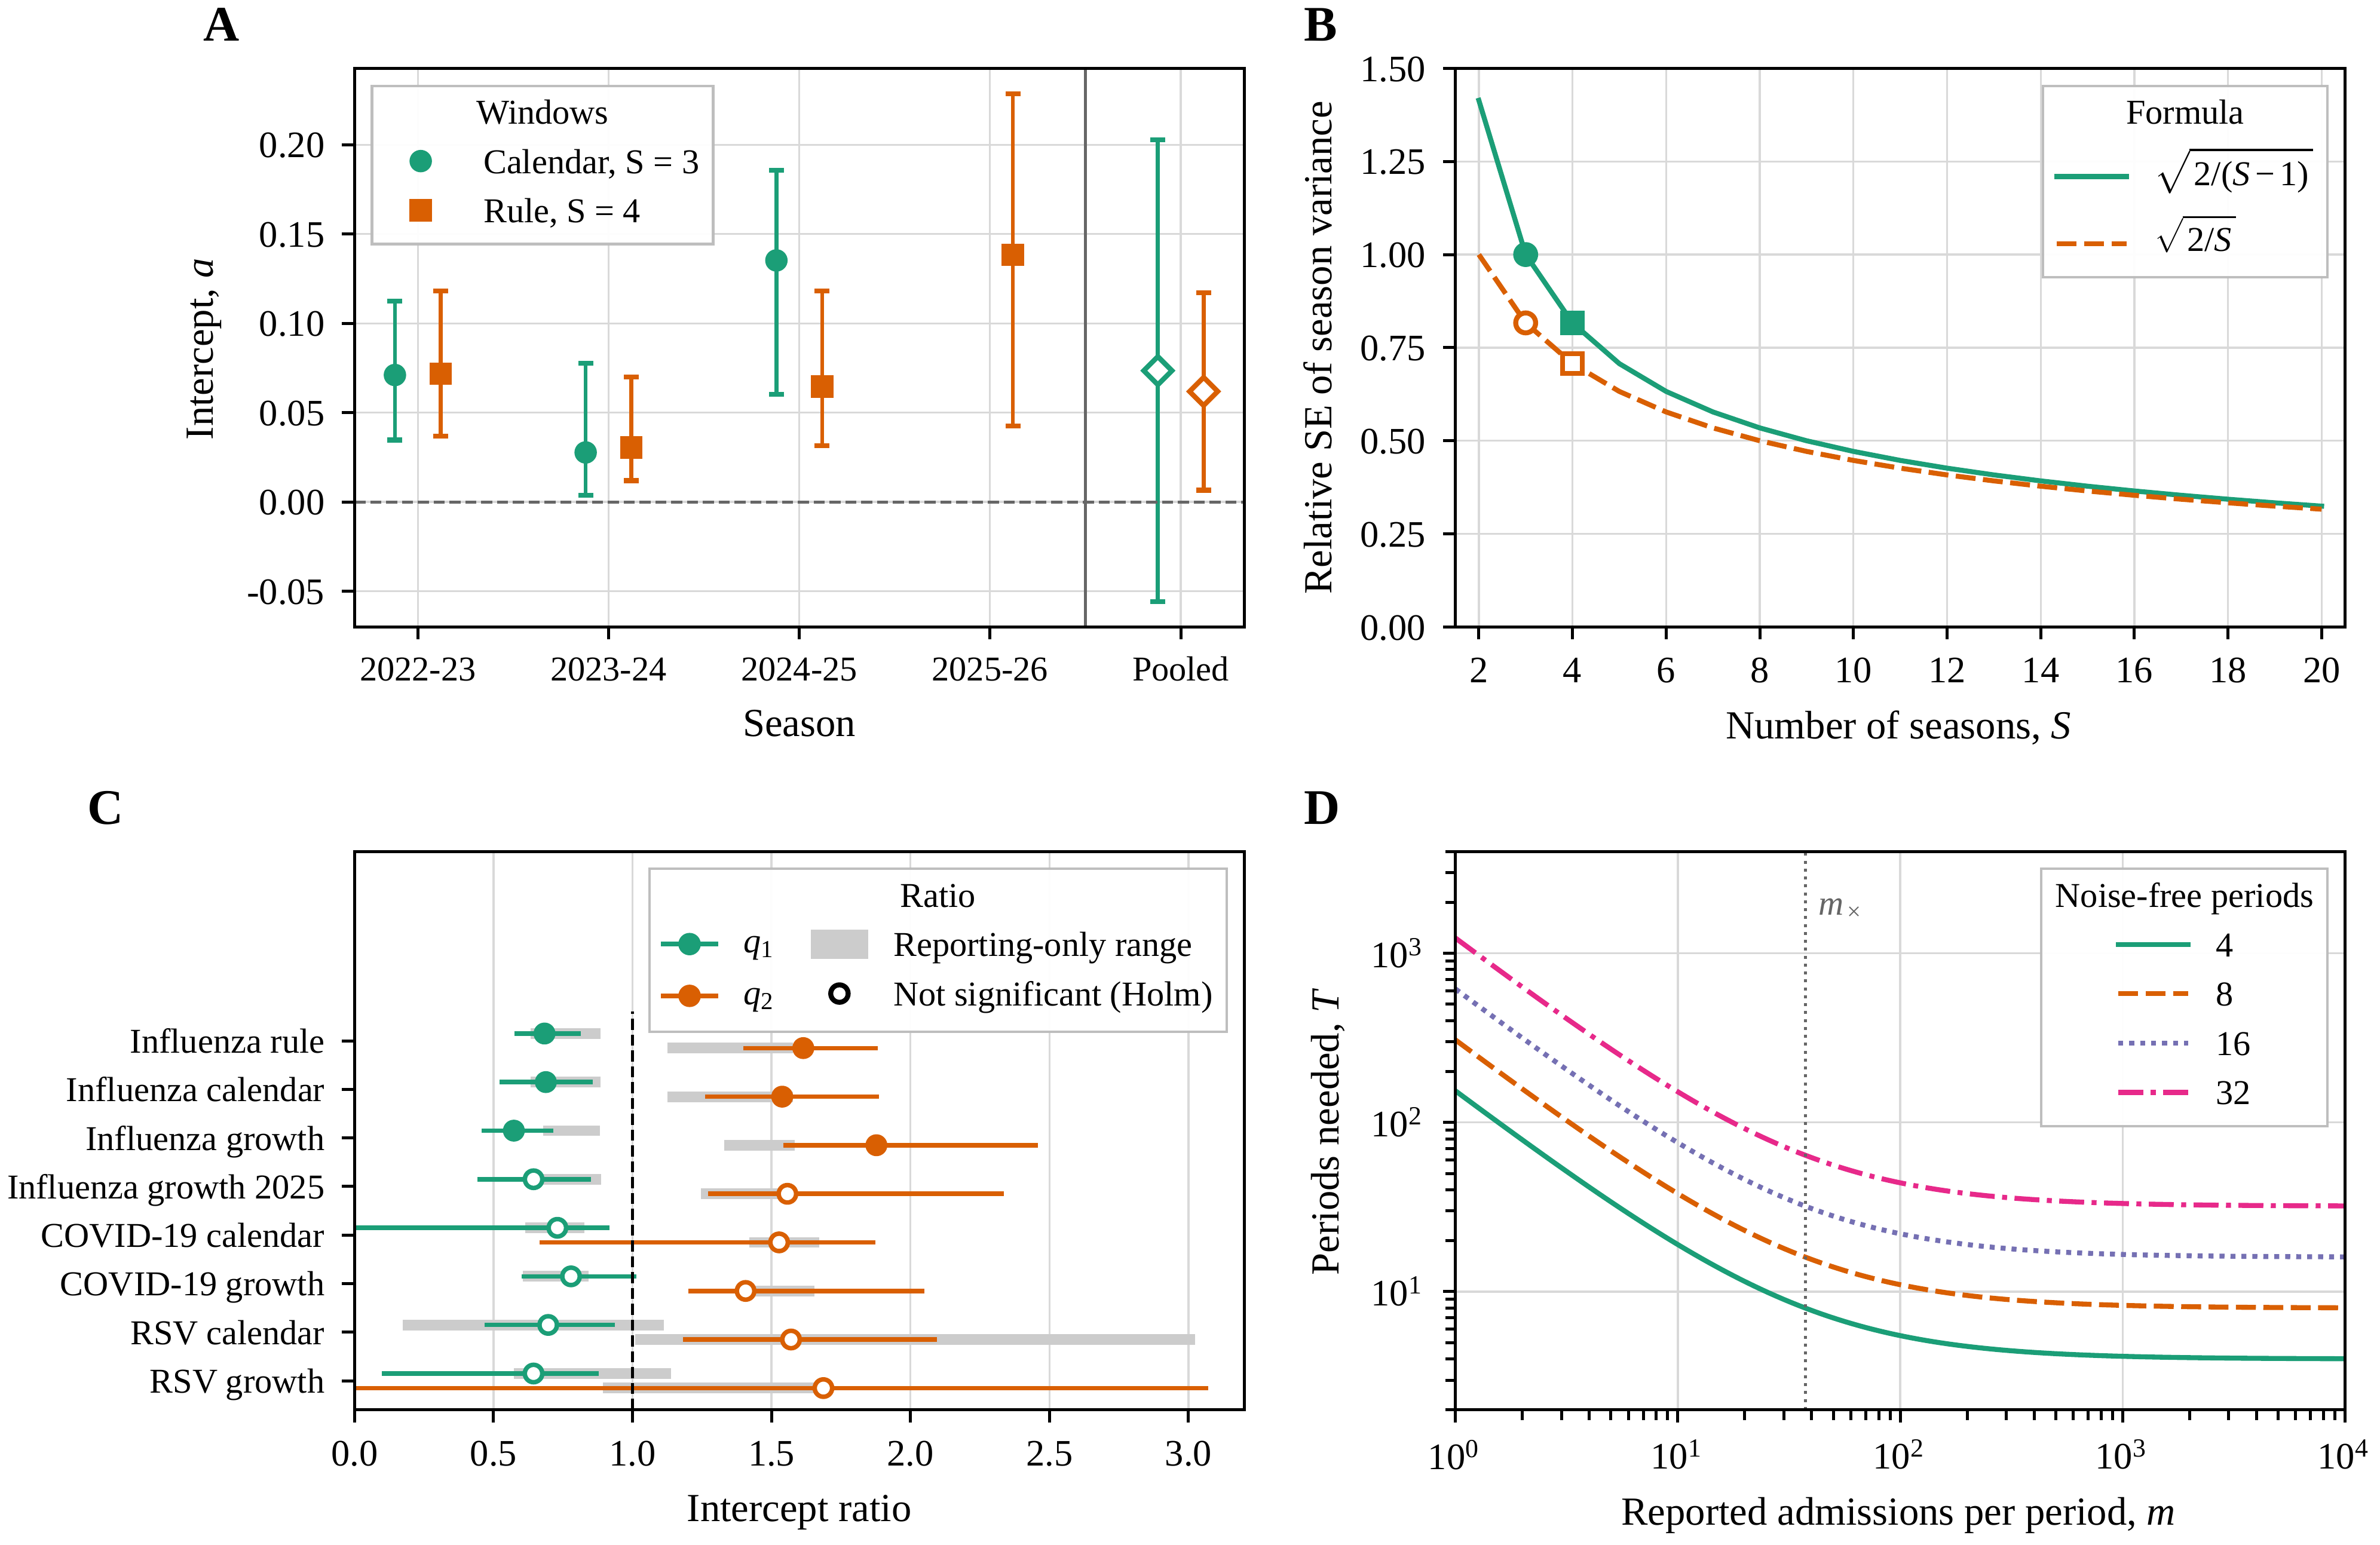
\includegraphics[width=0.86\linewidth]{figures/fig_07_seasons_pathogens_design.png}
  \caption{Between-season uncertainty, intercept ratios across pathogens and number of periods. (A) Season-specific intercepts of the weighted growth ratio in calendar windows and in rule-defined early-growth windows, with two-way bootstrap 95\% intervals; open diamonds show random-effects pooled estimates. Panel B gives the lower bound on the relative standard error of an estimated between-season variance against the number of seasons, compared with the values reported in the earlier analysis. Panel C gives intercept ratios for a single-week denominator and an equal three-week denominator relative to the original weights; grey bars give the ranges expected from reporting noise and epidemic growth without environmental variation, and filled markers denote one-sided tests that remain significant after Holm correction. Panel D gives the number of periods needed to match the precision of a given number of noise-free periods, by reported admissions per period; the panel is illustrative and is superseded by the empirical nomogram in Fig.~\ref{fig:design}A.}
  \label{fig:seasons}
\end{figure}

\FloatBarrier
\clearpage
\section{Supplementary tables}
\label{app:tables}

\setcounter{table}{0}
\renewcommand{\thetable}{S\arabic{table}}

Tables~\ref{tab:s1}--\ref{tab:s7} report the estimates that underlie Figs.~\ref{fig:floor}--\ref{fig:seasons}. Table~\ref{tab:s8} gives the implied environmental variance under each setting of the inversion (Fig.~\ref{fig:inversion}), and Table~\ref{tab:s9} lists the specifications used across the rounds of this analysis. Table~\ref{tab:s4} compares the voluntary reporting period with the same calendar months of the mandatory years. All values were generated from the stored outputs of the analysis code.

\begin{table}[htbp]
\centering
\footnotesize
\caption{Intercept $a$, slope $b$ and balance ratio $b/a$ of the relative loss by specification, with the two-way bootstrap 95\% confidence interval of each estimate.}
\label{tab:s1}
\begin{tabular}{lrrrlllr}
\toprule
Specification & $N$ & Weeks & $\bar{x}$ & $a$ [95\% CI] & $b$ [95\% CI] & $b/a$ [95\% CI] & SD ratio \\
\midrule
$R_A$, rule windows ($S=4$) & 1748 & 42 & 1.206 & 0.0150 [0.0100, 0.0208] & 0.560 [0.367, 0.769] & 37.4 [19.1, 71.0] & 1.95 \\
$G$, rule windows ($S=4$) & 1756 & 42 & 1.724 & 0.0840 [0.0498, 0.1248] & 1.971 [0.959, 3.098] & 23.5 [8.4, 59.7] & 2.29 \\
$G$, calendar windows ($S=3$) & 1267 & 29 & 1.671 & 0.0991 [0.0569, 0.1382] & 2.243 [1.060, 3.559] & 22.6 [9.0, 52.2] & 4.68 \\
$R_A$, calendar windows ($S=3$) & 1263 & 29 & 1.190 & 0.0202 [0.0097, 0.0306] & 0.516 [0.279, 0.839] & 25.6 [10.2, 79.6] & 3.46 \\
\bottomrule
\end{tabular}
\par\smallskip
\begin{minipage}{0.95\linewidth}\scriptsize Iterated FGLS fit of $L=((x-\bar{x})/\bar{x})^2$ on $a+b/D$; 95\% percentile intervals from the two-way (state $\times$ week) pigeonhole bootstrap, $B=2000$, $\bar{x}$ re-estimated in every replicate. SD ratio: bootstrap SD of $a$ under two-way versus state-only resampling. 51 jurisdictions throughout.\end{minipage}
\end{table}

\begin{table}[htbp]
\centering
\footnotesize
\setlength{\tabcolsep}{4pt}
\caption{Decomposition of the intercept and comparison of the affine model with a power law, with the 95\% confidence interval of each intercept.}
\label{tab:s2}
\begin{tabular}{lllrrrrrr}
\toprule
Specification & $a$ total & \begin{tabular}[t]{@{}c@{}}$a$ after\\ week effects\end{tabular} & \begin{tabular}[t]{@{}c@{}}$a$ after week and\\ state-season effects\end{tabular} & \begin{tabular}[t]{@{}c@{}}Week\\ share\end{tabular} & ICC & \begin{tabular}[t]{@{}c@{}}Power\\ exponent\end{tabular} & $p$ & \begin{tabular}[t]{@{}c@{}}CV folds\\ (state; season)\end{tabular} \\
\midrule
$R_A$, rule windows ($S=4$) & \begin{tabular}[t]{@{}c@{}}0.0150\\ \relax[0.0100, 0.0208]\end{tabular} & \begin{tabular}[t]{@{}c@{}}0.0088\\ \relax[0.0064, 0.0124]\end{tabular} & \begin{tabular}[t]{@{}c@{}}0.0083\\ \relax[0.0064, 0.0141]\end{tabular} & 0.41 & 0.25 & 0.38 & 0.11 & 26/51; 2/4 \\
$G$, rule windows ($S=4$) & \begin{tabular}[t]{@{}c@{}}0.0840\\ \relax[0.0508, 0.1226]\end{tabular} & \begin{tabular}[t]{@{}c@{}}0.0415\\ \relax[0.0306, 0.0586]\end{tabular} & \begin{tabular}[t]{@{}c@{}}0.0394\\ \relax[0.0293, 0.0614]\end{tabular} & 0.51 & 0.31 & 0.35 & 0.44 & 19/51; 0/4 \\
$G$, calendar windows ($S=3$) & \begin{tabular}[t]{@{}c@{}}0.0991\\ \relax[0.0583, 0.1399]\end{tabular} & \begin{tabular}[t]{@{}c@{}}0.0473\\ \relax[0.0337, 0.0676]\end{tabular} & \begin{tabular}[t]{@{}c@{}}0.0450\\ \relax[0.0335, 0.0932]\end{tabular} & 0.52 & 0.29 & 0.27 & 0.42 & 28/51; 3/3 \\
\bottomrule
\end{tabular}
\par\smallskip
\begin{minipage}{0.95\linewidth}\scriptsize Intervals are from a two-way bootstrap with $B=1000$; the draws are separate from those of Table S1, which explains small differences. The third column removes national week effects from the statistic before the fit, and the fourth also removes state-season effects. The week share equals one minus the ratio of the third to the second column. The ICC is the share of the variance of the statistic that lies between weeks. The power exponent is $c$ in $L=\alpha D^{-c}$, and $p$ is from a parametric-bootstrap test of the affine model against this power law with 200 null draws. CV folds counts the leave-one-state-out and leave-one-season-out folds in which the affine model predicts better. A power analysis found no fraction of the estimated $a$ ($\le 1$) detectable with 80\% power.\end{minipage}
\end{table}

\begin{table}[htbp]
\centering
\footnotesize
\caption{Equivalence tests for the contribution of facility-reporting completeness to the intercept, with the paired bootstrap 90\% confidence interval of each change.}
\label{tab:s3}
\begin{tabular}{llrlrlr}
\toprule
Specification & $10^3\Delta a$ [90\% CI] & $10^3\delta_{0.10}$ & Equiv. & $10^3\delta_{0.05}$ & Equiv. & Seasons equiv. \\
\midrule
$R_A$, rule windows ($S=4$) & 0.29 [$-$0.22, 0.85] & 2.55 & yes & 0.64 & no & 4/4 \\
$G$, rule windows ($S=4$) & 0.37 [$-$2.83, 2.81] & 10.13 & yes & 2.53 & no & 3/4 \\
$G$, calendar windows ($S=3$) & $-$0.38 [$-$3.55, 2.24] & 10.14 & yes & 2.54 & no & 2/3 \\
\bottomrule
\end{tabular}
\par\smallskip
\begin{minipage}{0.95\linewidth}\scriptsize $\Delta a$ is the intercept of the statistic minus that of the statistic recomputed from counts divided by the share of hospitals reporting, with a paired two-way bootstrap ($B=2000$). Margins $\delta_{\tau_0}=\kappa^2\tau_0^2(1+v_R/\bar{R}^2)$ were set from a reporting-volatility threshold and the sample mean $\bar{R}$ of each statistic ($\kappa=1$ for $G$, $v_R=0.04$). Equivalence is declared when the 90\% interval lies inside $(-\delta,\delta)$ (TOST, $\alpha=0.05$). The column of equivalent seasons counts seasons equivalent at $\tau_0=0.10$.\end{minipage}
\end{table}

\begin{table}[htbp]
\centering
\footnotesize
\caption{Calendar-matched comparison of the voluntary-reporting period (May--October).}
\label{tab:s4}
\begin{tabular}{llrll}
\toprule
Year & Reporting & $N$ & SD of $G$ & IQR of $\log G$ \\
\midrule
2023 & mandatory & 773 & 0.62 [0.40, 1.00] & 0.48 [0.40, 0.61] \\
2024 & voluntary & 420 & 1.82 [0.42, 4.10] & 0.76 [0.48, 1.04] \\
2025 & mandatory & 841 & 0.39 [0.33, 0.44] & 0.48 [0.37, 0.58] \\
\bottomrule
\end{tabular}
\par\smallskip
\begin{minipage}{0.95\linewidth}\scriptsize State-weeks with $D_t\ge 5$ whose week ends between 1 May and 31 October; 95\% two-way bootstrap intervals, $B=1000$. The FGLS intercept is not stable in the voluntary period (negative point estimate), so robust spread measures are reported. Laboratory proxy (Delphi FluView clinical laboratory data, 1224 state-weeks): share of the $R_A$ intercept shared with laboratory growth 0.23 [0.043, 0.42]; correlation 0.31 [0.19, 0.41].\end{minipage}
\end{table}

\begin{table}[htbp]
\centering
\footnotesize
\caption{Season-specific intercepts, each with its bootstrap 95\% confidence interval, and between-season heterogeneity, reported separately for $S=4$ and $S=3$.}
\label{tab:s5}
\begin{tabular}{llll}
\toprule
Season & $R_A$, rule windows ($S=4$) & $G$, rule windows ($S=4$) & $G$, calendar windows ($S=3$) \\
\midrule
2022-23 & 0.0137 [0.0066, 0.0213] & 0.0718 [0.0368, 0.1181] & 0.0711 [0.0347, 0.1124] \\
2023-24 & 0.0062 [0.0025, 0.0144] & 0.0305 [0.0119, 0.0700] & 0.0277 [0.0037, 0.0776] \\
2024-25 & 0.0127 [0.0057, 0.0241] & 0.0647 [0.0315, 0.1181] & 0.1352 [0.0602, 0.1857] \\
2025-26 & 0.0225 [0.0087, 0.0352] & 0.1383 [0.0426, 0.2285] & -- \\
$a_{\mathrm{RE}}$ [95\% CI] & 0.0125 [0.0022, 0.0227] & 0.0619 [0.0066, 0.1171] & 0.0735 [$-$0.0558, 0.2028] \\
$Q$ ($p$) & 5.71 (0.126) & 6.58 (0.087) & 8.92 (0.012) \\
$10^3\tau^2$ [Q-profile] & 0.019 [0.000, 0.599] & 0.620 [0.000, 26.756] & 2.077 [0.127, 114.859] \\
$I^2$ & 0.47 & 0.54 & 0.78 \\
\bottomrule
\end{tabular}
\par\smallskip
\begin{minipage}{0.95\linewidth}\scriptsize Season intercepts use the season's own mean; 95\% two-way bootstrap intervals, $B=1000$. DerSimonian--Laird random effects with a $t_{S-1}$ interval; Q-profile 95\% interval for $\tau^2$ \citep{viechtbauer2007confidence}. The relative standard error of a between-season variance estimated from $S$ seasons is at least $\sqrt{2/(S-1)}$: 1.00 for $S=3$ and 0.82 for $S=4$.\end{minipage}
\end{table}

\begin{table}[htbp]
\centering
\footnotesize
\setlength{\tabcolsep}{4pt}
\caption{Cross-pathogen intercept ratios against the pure-reporting growth null, with Holm-adjusted $p$-values.}
\label{tab:s6}
\begin{tabular}{lrllllrrrrr}
\toprule
Pathogen, window & $N$ & \begin{tabular}[t]{@{}c@{}}$q_1$\\ \relax[95\% CI]\end{tabular} & \begin{tabular}[t]{@{}c@{}}$q_2$\\ \relax[95\% CI]\end{tabular} & \begin{tabular}[t]{@{}c@{}}Null\\ $q_1$\end{tabular} & \begin{tabular}[t]{@{}c@{}}Null\\ $q_2$\end{tabular} & $q_1<1$ & $q_2>1$ & \begin{tabular}[t]{@{}c@{}}$q_1$\\ out\end{tabular} & \begin{tabular}[t]{@{}c@{}}$q_2$\\ out\end{tabular} & \begin{tabular}[t]{@{}c@{}}Excess\\ $>0$\end{tabular} \\
\midrule
Influenza, rule & 1756 & \begin{tabular}[t]{@{}c@{}}0.68\\ \relax[0.58, 0.81]\end{tabular} & \begin{tabular}[t]{@{}c@{}}1.61\\ \relax[1.41, 1.87]\end{tabular} & 0.63--0.89 & 1.13--1.58 & 0.020 & 0.034 & 1.000 & 1.000 & 0.034 \\
Influenza, calendar & 1267 & \begin{tabular}[t]{@{}c@{}}0.69\\ \relax[0.53, 0.85]\end{tabular} & \begin{tabular}[t]{@{}c@{}}1.54\\ \relax[1.27, 1.88]\end{tabular} & 0.63--0.89 & 1.13--1.58 & 0.020 & 0.020 & 1.000 & 1.000 & 0.020 \\
Influenza, growth & 2707 & \begin{tabular}[t]{@{}c@{}}0.57\\ \relax[0.47, 0.71]\end{tabular} & \begin{tabular}[t]{@{}c@{}}1.88\\ \relax[1.55, 2.45]\end{tabular} & 0.68--0.88 & 1.33--1.58 & 0.034 & 0.020 & 1.000 & 1.000 & 0.020 \\
Influenza, growth, 2025-26 & 663 & \begin{tabular}[t]{@{}c@{}}0.64\\ \relax[0.45, 0.84]\end{tabular} & \begin{tabular}[t]{@{}c@{}}1.56\\ \relax[1.28, 2.33]\end{tabular} & 0.66--0.89 & 1.25--1.57 & 0.116 & 0.075 & 1.000 & 1.000 & 0.046 \\
COVID-19, calendar & 1479 & \begin{tabular}[t]{@{}c@{}}0.73\\ \relax[n.d., 0.91]\end{tabular} & \begin{tabular}[t]{@{}c@{}}1.53\\ \relax[0.67, 1.87]\end{tabular} & 0.61--0.83 & 1.42--1.67 & 0.287 & 0.616 & 1.000 & 1.000 & 1.000 \\
COVID-19, growth & 2862 & \begin{tabular}[t]{@{}c@{}}0.78\\ \relax[0.61, 1.01]\end{tabular} & \begin{tabular}[t]{@{}c@{}}1.41\\ \relax[1.21, 2.04]\end{tabular} & 0.60--0.84 & 1.40--1.66 & 0.616 & 0.154 & 1.000 & 1.000 & 1.000 \\
RSV, calendar & 494 & \begin{tabular}[t]{@{}c@{}}0.70\\ \relax[0.48, 0.93]\end{tabular} & \begin{tabular}[t]{@{}c@{}}1.57\\ \relax[1.19, 2.09]\end{tabular} & 0.17--1.11 & 1.01--3.02 & 0.154 & 0.228 & 1.000 & 1.000 & 0.200 \\
RSV, growth & 1073 & \begin{tabular}[t]{@{}c@{}}0.64\\ \relax[0.11, 0.87]\end{tabular} & \begin{tabular}[t]{@{}c@{}}1.69\\ \relax[n.d., 3.06]\end{tabular} & 0.57--1.14 & 0.89--1.69 & 0.182 & 0.660 & 1.000 & 1.000 & 1.000 \\
\bottomrule
\end{tabular}
\par\smallskip
\begin{minipage}{0.95\linewidth}\scriptsize Here $q_1=a_{\text{1 week}}/a_{\text{original}}$ and $q_2=a_{\text{equal 3 weeks}}/a_{\text{original}}$, with intervals from a shared two-way bootstrap ($B=2000$). Null ranges come from a growth-null simulation without transmission heterogeneity over three generation intervals, three admission delays and four reporting-noise levels; the rule-window row uses the influenza calendar range. The last five columns give one-sided bootstrap $p$-values, Holm-adjusted over all 40 tests, and the columns marked out test whether the ratio lies outside the null range. Excess denotes $a-v_R/\bar{G}^2$ with $v_R=0.04$. A lower bound marked n.d. is not defined because some bootstrap replicates gave a negative intercept in the ratio, so the ratio has no positive lower limit; the upper limit is shown as estimated.\end{minipage}
\end{table}

\begin{table}[htbp]
\centering
\footnotesize
\caption{Theory quantities recomputed from the closed forms and compared with an earlier version of this analysis.}
\label{tab:s7}
\begin{tabular}{lrrl}
\toprule
Quantity & Earlier & Recomputed & Status \\
\midrule
$m_\times$ & 53.1 & 53.08 & reproduced \\
$v_H$ ($\tau=0.15$) & 0.0307 & 0.0307 & reproduced \\
$m_{\times,H}$ ($\tau=0.15$) & 30.4 & 30.36 & reproduced \\
$m_0^*$ ($c_0/c_1=100$) & 72.9 & 72.86 & reproduced \\
$T^\dagger$ ($\phi=0.8$) & 4.48 & 4.484 & reproduced \\
$B^\dagger$ & 775 & 775.0 & reproduced \\
$B^\dagger$ ($m_\times=21.3$) & 655 & 655.3 & reproduced \\
$B^\dagger$ ($m_\times=49.2$) & 763 & 762.9 & reproduced \\
Reporting lever term ($\times10^{-3}$) & 7.85 & 7.88 & corrected \\
Lever total ($\times10^{-3}$) & 22.5 & 22.57 & corrected \\
Fisher constant & 0.505 & 0.505 & reproduced \\
Relative SE, $S=3$ & 0.82 & 1.000 & corrected \\
Relative SE, $S=4$ & 0.71 & 0.816 & corrected \\
\bottomrule
\end{tabular}
\par\smallskip
\begin{minipage}{0.95\linewidth}\scriptsize Baseline $\bar{R}=1.15$, $v_R=0.04$, $k=0.35$, $\rho=0.25$. The earlier relative standard errors for $S=3,4$ equal $\sqrt{2/S}$; the stated bound $\sqrt{2/(S-1)}$ gives the recomputed values. The lever terms differ by rounding.\end{minipage}
\end{table}

\begin{table}[htbp]
\centering
\footnotesize
\setlength{\tabcolsep}{4pt}
\caption{Implied environmental variance $v_R^{\mathrm{impl}}$ from the two-step inversion under each simulation setting, with the 95\% confidence interval of each estimate.}
\label{tab:s8}
\begin{tabular}{lllrrll}
\toprule
Setting & $v_R^{\mathrm{impl}}$ from $R_A$ & $v_R^{\mathrm{impl}}$ from $G$ & $\kappa_{R_A}$ & $\kappa_G$ & Ratio $R_A/G$ & Agree \\
\midrule
Data-matched design (M0) & 0.040 [0.026, 0.056] & 0.043 [0.025, 0.064] & 0.516 & 2.729 & 0.93 [0.78, 1.18] & yes \\
No national shock & 0.039 [0.026, 0.055] & 0.042 [0.024, 0.062] & 0.523 & 2.775 & 0.94 [0.79, 1.18] & yes \\
National share 0.65 & 0.040 [0.026, 0.056] & 0.043 [0.025, 0.065] & 0.510 & 2.670 & 0.92 [0.77, 1.16] & yes \\
AR(1), $\phi=0.5$ & 0.027 [0.017, 0.040] & 0.025 [0.013, 0.039] & 0.780 & 4.699 & 1.08 [0.88, 1.43] & yes \\
True GI mean 2.2 d & 0.013 [0.008, 0.019] & 0.014 [0.008, 0.021] & 1.287 & 6.991 & 0.94 [0.77, 1.20] & yes \\
True GI mean 4.3 d & 0.058 [0.038, 0.081] & 0.063 [0.037, 0.095] & 0.380 & 1.977 & 0.92 [0.77, 1.16] & yes \\
Delay mean 3.5 d & 0.038 [0.025, 0.053] & 0.041 [0.024, 0.061] & 0.535 & 2.790 & 0.93 [0.77, 1.16] & yes \\
Delay mean 8 d & 0.046 [0.030, 0.064] & 0.047 [0.027, 0.069] & 0.454 & 2.483 & 0.98 [0.82, 1.22] & yes \\
$k=0.1$ & 0.040 [0.026, 0.055] & 0.042 [0.025, 0.062] & 0.517 & 2.740 & 0.94 [0.79, 1.18] & yes \\
Synchronous count shock & 0.019 [0.006, 0.035] & 0.029 [0.012, 0.048] & 1.041 & 4.553 & 0.67 [0.39, 0.90] & no \\
Generic design (bridge) & 0.043 [0.029, 0.059] & 0.044 [0.027, 0.063] & 0.507 & 2.734 & 0.97 [0.83, 1.18] & -- \\
\bottomrule
\end{tabular}
\par\smallskip
\begin{minipage}{0.95\linewidth}\scriptsize Each setting changes one element of the data-matched design (Section~\ref{sec:meth-inversion}); the analyst's generation interval stays at a mean of 3.6 days throughout. Intervals combine 2000 joint two-way bootstrap draws of the two empirical intercepts with draws of the calibration line from its Monte Carlo sampling distribution. $\kappa=\E(\hat{a})/(v_R/\bar{R}^2)$ at the grid value of $v_R$ nearest to the implied variance. Agree marks settings in which the 95\% interval of the difference between the two implied variances contains zero; the generic design of the first simulation is shown as a bridge and is not counted among the ten settings.\end{minipage}
\end{table}

\begin{table}[htbp]
\centering
\footnotesize
\setlength{\tabcolsep}{4pt}
\caption{Specifications used across the rounds of this analysis, with the 95\% confidence interval of each estimate on the data version of 2026-10-20.}
\label{tab:s9}
\begin{tabular}{p{0.27\linewidth}p{0.22\linewidth}ll}
\toprule
Round and specification & Role & $a$ [95\% CI] & $b/a$ [95\% CI] \\
\midrule
Round 1: $G$, three calendar windows ($S=3$) & Primary in round 1; secondary from round 2 & 0.0991 [0.0569, 0.1382] & 22.6 [9.0, 52.2] \\
Round 2, rule version 1: windows ending at the season maximum & Abandoned (four weeks in 2024--25); no estimates retained & -- & -- \\
Round 2, rule version 2 (2026-10-20): $G$, rule windows ($S=4$) & Secondary & 0.0840 [0.0498, 0.1248] & 23.5 [8.4, 59.7] \\
Round 2, rule version 2: $R_A$, rule windows ($S=4$) & Primary from round 2 & 0.0150 [0.0100, 0.0208] & 37.4 [19.1, 71.0] \\
Round 2: $R_A$, calendar windows ($S=3$) & Sensitivity & 0.0202 [0.0097, 0.0306] & 25.6 [10.2, 79.6] \\
Round 3: two-step inversion & Calibration of the round-2 fits; no refit & -- & -- \\
\bottomrule
\end{tabular}
\par\smallskip
\begin{minipage}{0.95\linewidth}\scriptsize All estimates were refitted on the same data version with two-way bootstrap intervals ($B=2000$). The renewal-type ratio became the primary statistic in round 2 because its relationship to $R_t$ is explicit through the generation interval; the weighted growth ratio is retained for continuity. The point estimate of each specification lies inside the interval of the other specification of the same statistic.\end{minipage}
\end{table}

\begin{table}[htbp]
\centering
\footnotesize
\setlength{\tabcolsep}{4pt}
\caption{Lag-1 autocorrelation, and implied environmental variance and $b/a$ in the added inversion settings.}
\label{tab:s10}
\begin{tabular}{lllll}
\toprule
\multicolumn{5}{l}{\textit{A. Lag-1 autocorrelation}}\\
Setting & $r_1$ of $R_A$ & Data pct. & $r_1$ of $G$ & Data pct. \\
\midrule
Data (rule windows) & $-$0.095 [$-$0.168, $-$0.019] & -- & 0.123 [0.039, 0.201] & -- \\
Data-matched design (M0) & $-$0.074 [$-$0.151, 0.014] & 31.0 & 0.114 [0.025, 0.220] & 62.0 \\
AR(1), $\phi=0.25$ & 0.007 [$-$0.098, 0.118] & 3.0 & 0.193 [0.097, 0.304] & 10.0 \\
AR(1), $\phi=0.5$ & 0.072 [$-$0.039, 0.229] & 0.0 & 0.258 [0.146, 0.390] & 0.0 \\
True GI mean 2.2 d & 0.099 [$-$0.002, 0.223] & 0.0 & 0.251 [0.156, 0.363] & 0.0 \\
True GI mean 2.9 d & 0.006 [$-$0.083, 0.120] & 2.5 & 0.183 [0.091, 0.296] & 9.0 \\
True GI mean 4.3 d & $-$0.134 [$-$0.206, $-$0.030] & 80.0 & 0.051 [$-$0.031, 0.161] & 92.0 \\
Admissions VMR 1.5 & $-$0.170 [$-$0.233, $-$0.096] & 97.5 & $-$0.014 [$-$0.092, 0.076] & 100.0 \\
Admissions VMR 2.0 & $-$0.183 [$-$0.247, $-$0.104] & 99.0 & $-$0.041 [$-$0.104, 0.035] & 100.0 \\
Synchronous count shock & $-$0.146 [$-$0.225, $-$0.076] & 86.0 & 0.041 [$-$0.033, 0.116] & 99.0 \\
\midrule
\multicolumn{5}{l}{\textit{B. Added settings ($b/a$ pooled at $v_R=0.04$)}}\\
Setting & $v_R^{\mathrm{impl}}$ from $R_A$ & $v_R^{\mathrm{impl}}$ from $G$ & $b/a$ of $R_A$ & $b/a$ of $G$ \\
\midrule
Data-matched design (M0) & 0.040 [0.026, 0.056] & 0.043 [0.025, 0.064] & 28.0 & 16.2 \\
True GI mean 2.9 d & 0.026 [0.017, 0.036] & 0.027 [0.016, 0.040] & 18.2 & 10.4 \\
Admissions VMR 1.5 & 0.039 [0.026, 0.055] & 0.044 [0.026, 0.066] & 68.0 & 40.2 \\
Admissions VMR 2.0 & 0.039 [0.026, 0.055] & 0.045 [0.027, 0.066] & 81.0 & 48.4 \\
AR(1), $\phi=0.25$ & 0.033 [0.021, 0.047] & 0.033 [0.019, 0.049] & 23.4 & 12.6 \\
\bottomrule
\end{tabular}
\par\smallskip
\begin{minipage}{0.95\linewidth}\scriptsize $r_1$ is the pooled lag-1 autocorrelation of the relative deviation $x/\bar{x}_{\mathrm{block}}-1$ within state-season blocks. The interval for the data comes from a state-cluster bootstrap with 1000 draws; simulated rows give the mean and the 2.5\% to 97.5\% range of $r_1$ over panels at $v_R=0.04$ (200 panels per value of $v_R$ for the added settings, 100 for the others), and Data pct.\ is the percentile of the empirical value in that distribution. The analyst's generation interval stays at a mean of 3.6 days; 2.9 and 4.3 days are the ends of the 95\% interval for the serial interval of influenza in \citet{cowling2009estimation}. Overdispersed admissions use a gamma--Poisson mixture on weekly counts.\end{minipage}
\end{table}

